\documentclass[12pt,letterpaper]{article}
\usepackage[margin=1in]{geometry}
\usepackage[intlimits]{amsmath}
\usepackage{graphicx}
\usepackage{fancybox}
\usepackage{ifthen}
\usepackage{url}
\usepackage{lscape,afterpage}
\usepackage{xspace}
\usepackage{epstopdf} 
\usepackage{subcaption}
\graphicspath{{Figures/}}
\begin{document}
\title{Technical Note: $^{11}$C Spallation Production Measurement}
\author{Hasung Song}
\maketitle
\begin{abstract}
	This technical note describes the $^{11}$C measurement in KLZ and how the rate is extracted.
\end{abstract}

\subsection*{Spallation Event Selection}
\begin{itemize}
	\item FBE muon selection cuts
	\item MoGURA neutron selection cuts
	\item Neutron Shower Cuts ($N_n=1$)
	\item $^{11}$C Candidate cuts
	\begin{itemize}
		\item Energy Range
		\item FBE Run Start Delay
		\item Radius
	\end{itemize}
	\item $dR$ Cut 
\end{itemize}

\subsection*{Fit to $dT$}
dT of muon-event pairs where the neutron shower contained 1 observed neutron is shown in Figure \ref{fig:dT_fits}.
\begin{figure}[h]
	\centering
	\subcaptionbox{XeLS\label{fig:dT_XeLS}}[0.45\textwidth]{
		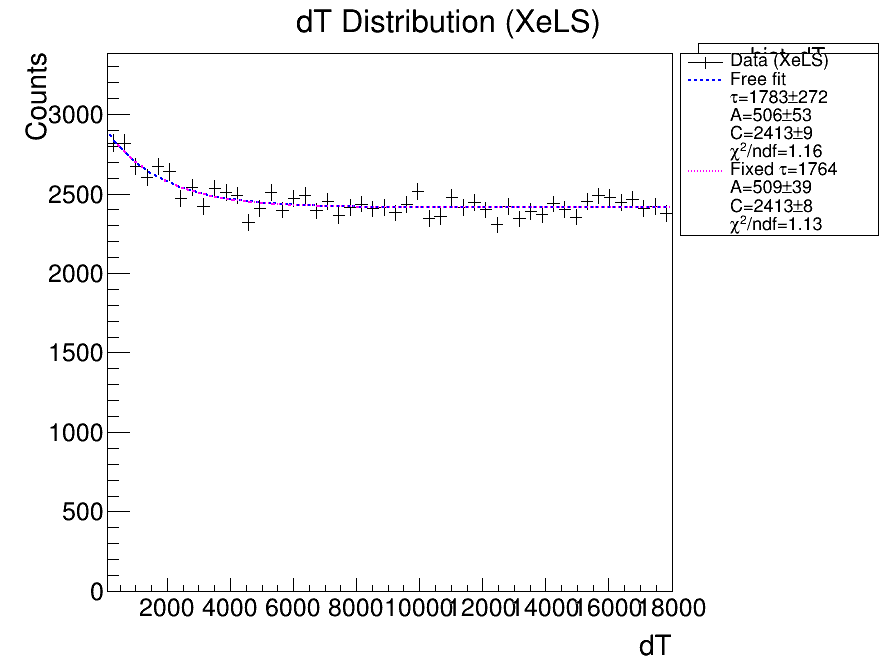
\includegraphics[width=0.45\textwidth]{dT_distribution_allcuts_XeLS.png}}
	\hfill
	\subcaptionbox{KamLS\label{fig:dT_KamLS}}[0.45\textwidth]{
		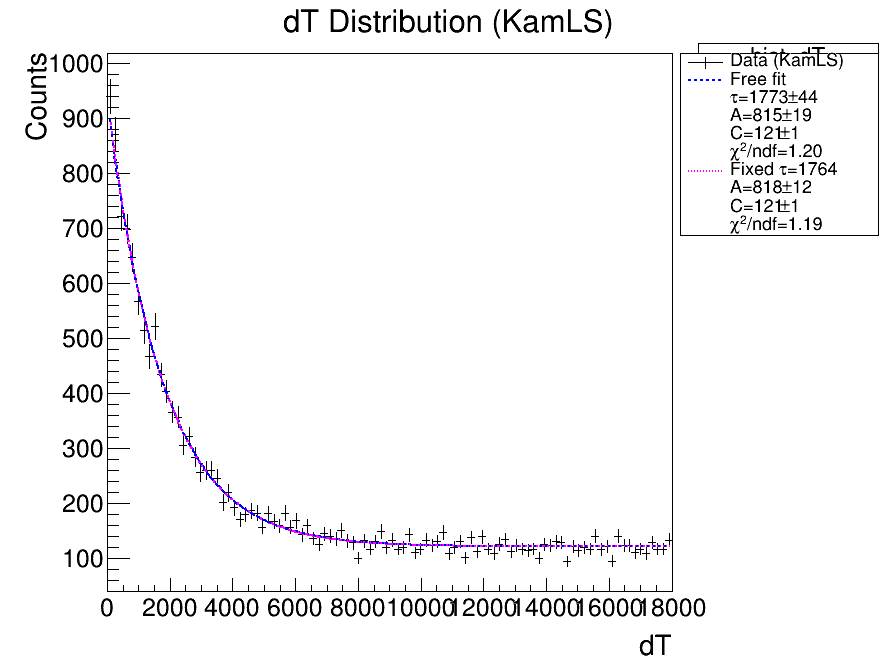
\includegraphics[width=0.45\textwidth]{dT_distribution_allcuts_KamLS.png}}
	\caption{dT of muon-event pairs where the neutron shower contained 1 observed neutron.}
	\label{fig:dT_fits}
\end{figure}

\subsection*{Rate Calculation}
\begin{itemize}
	\item Exposure, Livetime
	\item MoGURA Deadtime 
	\begin{itemize}
		\item simply scale up based on the deadtime since muons that occur during deadtime will not be able to create accurate pairs.
		\item Have to go through the MoGURA/FBE runs and check for overlap. (May be some function of the integral of $^{11}$C half-life?)
	\end{itemize}
	\item Neutron Production : How many muons that create $^{11}$C create exactly 1 \textbf{observed} neutron
	\begin{itemize}
		\item Muons that create $^{11}$C and create $1+$ neutrons, some fraction of those have only one detected (Toy MC calculation using Neutron Tagging Efficiency)
		\item The rate of muons creating other isotopes is not important, because those are not in the "good" exponential distribution of $\mu-^{11}$C pairs.
	\end{itemize}
	\item dR cut efficiency (from FLUKA tuned with $^{11}$C), for each data period\
	\item Fiducial Volume Cut Efficiency (from MC)
	\item Energy Cut Efficiency
\end{itemize}

\subsection*{Systematic Errors}
\begin{itemize}
	\item Exposure Uncertainty, from theses FV uncertainty ~4\%
	\item Neutron Tagging Efficiency Error: $74.5\%\pm0.4\%$
	\item FLUKA simulation Systematic : dR Cut, Neutron Production
	\item FLUKA simulation Statistical (small)
	\item Energy Scale Uncertainty? (use 1 sigma of kB, R contour)
\end{itemize}

\subsection*{Result}


\end{document}